\documentclass{article}
% \renewcommand{\familydefault}{\sfdefault}
\usepackage[a4paper, total={6in, 8in}]{geometry}
\usepackage{listings}
\usepackage{color}
\usepackage{tikz}
\usepackage{courier}
\usepackage{pgf-umlcd}
\usepackage{anyfontsize}

\newcommand{\NA}{---}

\title{Dark Forest NEA Project Report}
\author{Ethan Brierley}

\begin{document}
\maketitle
\newpage

\tableofcontents
\newpage

\section{Introduction}

\subsection{Motivation}

This project is based around the popular early 1980s phenomenon of the choose your own adventure game books.
Dark Forest aims to create a unified digital platform for the creating, sharing and playing of games build with a similar structure.

\subsection{Iteration}

This project was managed under a Git repository for version control.
This resulted in a full project history showing the iteration of over 200 commits created over more than 5 months.



\lstset{basicstyle=\tiny}
\lstinputlisting{gitlog}

\lstset{basicstyle=\normalsize}
The output of the command \texttt{git log --graph --oneline}

% https://tex.stackexchange.com/questions/125244/how-can-i-produce-the-history-graph-of-a-git-repository-in-latex/156501

\section{Technology}

\section{Project Structure}

To better organize the various components that make up Dark Forest the code was split into three independent libraries.
This acts as a form of stepwise refinement at the highest level.

\begin{center}
    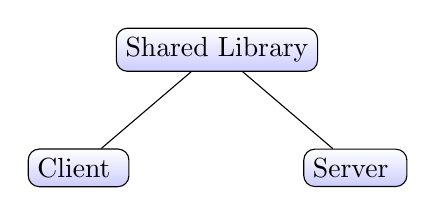
\begin{tikzpicture}[sibling distance=10em,
            every node/.style = {shape=rectangle, rounded corners,
                    draw, align=center,
                    top color=white, bottom color=blue!20}]]
        \node {Shared Library}
        child { node { Client } }
        child { node { Server } };
    \end{tikzpicture}
\end{center}

The client and server components both produce forms of executables to be independently run and to communicate over HTTP.

\subsection{Shared}

The shared library acts a dependency of both client and server and defines common interfaces used by both.

The shared library defines all types serialized, deserialized and sent over HTTP along with other types required by both the client and server

\subsubsection{API Endpoint Interfaces}

The Shared library defines two interfaces for Endpoints.
\texttt{Endpoint} for requests that do not have a body, namely requests using the HTTP verb GET.
\texttt{PostEndpoint} for requests that require a body of some form, namely requests using the verb POST.

Because of the fact that \texttt{PostEndpoint} inherits from \texttt{Endpoint} there is a type that implements \texttt{Endpoint} for each API facing endpoint.

The associated types \texttt{Response} and \texttt{Requires} both implement serialize and deserialize from the serde crate.
This ensures that it is always possible to transmit said types via a variety of methods.

\begin{center}
    \resizebox{200pt}{200pt}{
        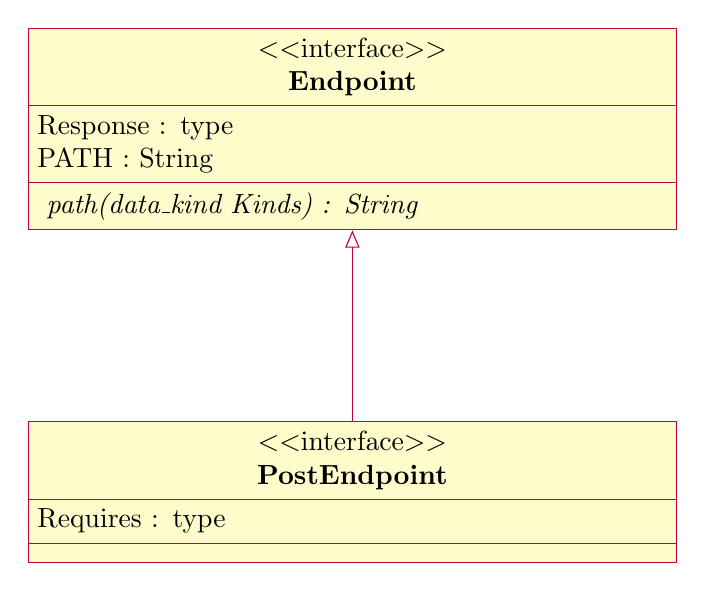
\begin{tikzpicture}
            \begin{interface}[text width=8cm]{Endpoint}{0,0}
                \attribute{Response : type}
                \attribute{PATH : String}
                \operation [0]{ path(data\_kind  Kinds) : String}
            \end{interface}
            \begin{interface}[text width=8cm]{PostEndpoint}{0,-5}
                \inherit{Endpoint}
                \attribute{Requires : type}
            \end{interface}

        \end{tikzpicture}
    }
\end{center}

\subsubsection{API Endpoints}

\begin{table}[h!]
    \small
    \begin{center}
        \label{tab:table1}
        \begin{tabular}{c|c|c|c|c}
            \textbf{Path}            & \textbf{Response}            & \textbf{Requires}               & \textbf{Descrption}                \\
            \hline
            \texttt{/hello}          & \texttt{Res}                 & \NA                             & Testing endpoint                   \\
            \texttt{/create-account} & \texttt{Result<(), Fail>}    & \texttt{Details}                & Creating a user account            \\
            \texttt{/new-protect}    & \texttt{Result<(), Fail>}    & \texttt{Authenticated<Details>} & Creating new games                 \\
            \texttt{/refresh-token}  & \texttt{Option<Token>}       & \texttt{Token}                  & Generating a new token             \\
            \texttt{/sign-in}        & \texttt{Result<Token, Fail>} & \texttt{Credential}             & Signing in a user with credentials \\
            \texttt{/signed-in}      & \texttt{Res}                 & \texttt{Token}                  & Check if a user is signed in       \\
        \end{tabular}
    \end{center}
\end{table}
\subsubsection{User Facing Endpoints}

\subsection{Server}
\subsection{Client}

\section{Login and Security}

\section{Building and running}
\section{Telemetry and logging}
\section{Data Structures}
\subsection{A Game as a Multigraph}
The core data structure in Dark Forest is a multigraph.
A multigraph is a form of graph where multiple edges can exist between two nodes.

In the case of this program the multigraph exists as a mutable user defined finite state machine.
The state machine is traversed during the "play" stage.
The states are game states and the transitions are choices that the player makes.

In our case we have more of a Mealy machine as there are two accepting states.
The case that the user "wins" and the "losing" state.

\section{Database}

\end{document}
